\documentclass[a4paper,10pt]{article}
\usepackage[a4paper, margin=0.5in]{geometry}
\usepackage{graphicx}
\usepackage{titlesec}
\usepackage{fontspec}
\usepackage{enumitem}
\usepackage{multicol}
\usepackage{hyperref}
\usepackage{fontawesome5}

\setmainfont{Arial}

% Define colors
\usepackage{xcolor}
\definecolor{primary}{RGB}{34, 139, 34}
\definecolor{secondary}{RGB}{102, 102, 102}

% Title formatting
\titleformat{\section}{\large\bfseries\color{primary}}{}{0em}{}
\titlespacing{\section}{0pt}{1em}{0.5em}

% Subtitle formatting
\titleformat{\subsection}{\normalsize\bfseries\color{secondary}}{}{0em}{}
\titlespacing{\subsection}{0pt}{0.5em}{0.25em}

% No indentation
\setlength{\parindent}{0pt}

% Small space between paragraphs
\setlength{\parskip}{0.5em}

% Link color
\hypersetup{
    colorlinks=true,
    linkcolor=primary,
    urlcolor=primary
}

\begin{document}

% Header
\begin{minipage}{0.65\textwidth}
    \vspace{0.2in}
    \Huge \textbf{Khandoker Sefayet Alam} \\
    \large Competitive Programmer \& MERN stack developer \\
    \vspace{0.1in}
    \normalsize
    \begin{tabbing}
    \hspace{2in} \= \hspace{3in} \kill
    \faPhone \ \texttt{+8801919030974} \> \faMapMarker* \ Rajshahi, Bangladesh \\
    \faEnvelope \ \texttt{sefayetalem14@gmail.com} \> \faGlobe \ \href{https://sefayet.xyz}{sefayet.xyz} \\
    \end{tabbing}
\end{minipage}
\begin{minipage}{0.3\textwidth}
    \raggedleft
    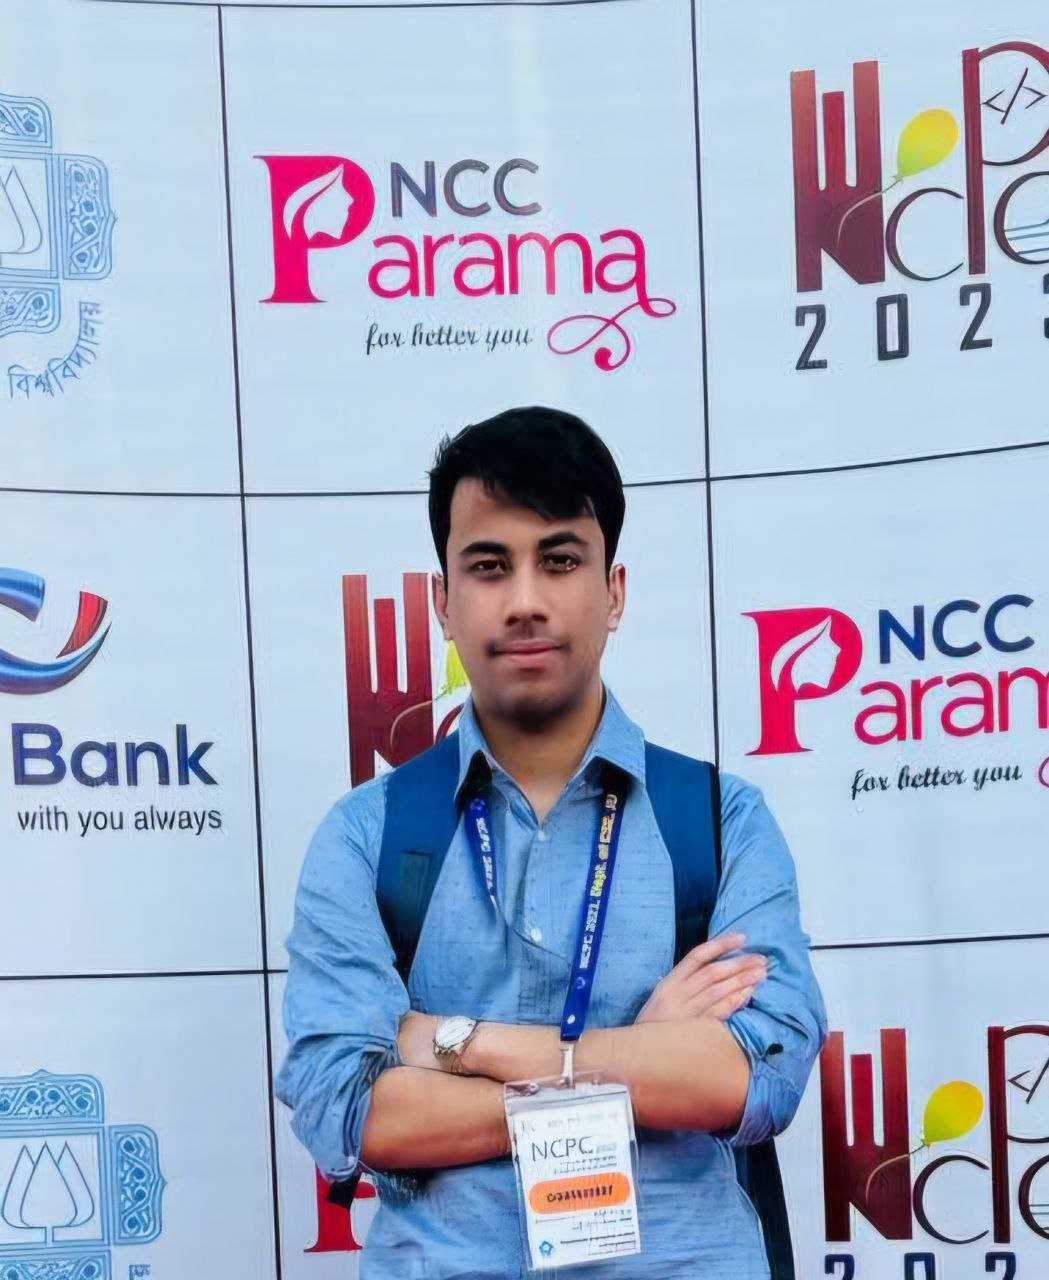
\includegraphics[width=1.2in]{image.png} % Add your image here
\end{minipage}

% Two columns layout
\begin{multicols}{2}

% Summary section
\section*{SUMMARY}
A dedicated undergraduate student pursuing a B.Sc in Computer Science and Engineering at RUET, specializing in full-stack development with the MERN stack and backend frameworks like Django. Proficient in JavaScript and Python, with expertise in building scalable web applications and integrating machine learning concepts. Experienced in competitive programming and adept at solving complex problems. Seeking to apply skills in a dynamic professional environment.

% Experience section
\section*{EXPERIENCE}
\textbf{Title} \\
Company Name \\
\textit{Date period} \\
Location \\
\textit{Company Description} \\
\begin{itemize}[noitemsep]
    \item Put achievements match
\end{itemize}

\textbf{Project name} \\
Description

% Education section
\section*{EDUCATION}
\textbf{B.Sc in Computer Science and Engineering} \\
Rajshahi University of Engineering and Technology \\
2022 - 2025

% Personal projects section
\section*{PERSONAL PROJECTS}
\textbf{Food App} \\
2024 - 2024 \\
Developed a Food App using React and a food API, enabling users to search and browse detailed cooking instructions, ingredients, and dietary information. \\
\textit{Utilized: React and Food APIs}

\textbf{Web development Course Manager} \\
2024 - 2024 \\
RUET \\
Developed a web application using React and Django, facilitating efficient project management for teachers. Features include authentication for secure access, project CRUD operations, and tracking project details like start dates, end dates, statuses, and comments. \\
\textit{Utilized: Django, Django-REST-framework, React}

% Languages section
\section*{LANGUAGES}
\textbf{English} \\
Proficient

\textbf{Bangla} \\
Native

% Achievements section
\section*{ACHIEVEMENTS}
\begin{enumerate}[noitemsep]
    \item Code Samurai 2024 Finalist \\
    \textit{RUET\_UNKNOWNS team qualified for onsite contest in 2024}
    \item CODESPARK 2022: 1st Runners Up \\
    \textit{Intra RUET freshers team programming contest}
    \item NCPC finalist 2023 \\
    \textit{RUET\_Chunins qualified for NCPC 2023}
    \item Codesmash 2021: 2nd Runners Up \\
    \textit{Intra RUET fresher’s programming contest}
    \item IUT ICT Fest: IUT IUPC 2024 \\
    \textit{RUET\_Onirban secured the place 20th in IUT IUPC 2024}
    \item Meta Hacker Cup \\
    \textit{Participated in Meta Hacker Cup 2023 Round 3 and secured the 1357th position out of 6193 coders}
    \item Problem Setter of Codesmash 2022 \\
    \textit{Set interesting problem for RUET intra freshers programming contest}
\end{enumerate}

% Training / Courses section
\section*{TRAINING / COURSES}
\textbf{Bible of Competitive Programming and Coding Interviews} \\
Udemy

\textbf{Full Stack Development with MERN} \\
Ostad

% Publications section
\section*{PUBLICATIONS}
\textbf{XYZ} \\
RUET

\textbf{AbC} \\
2024 - 2024 \\
\textit{Publication Description}

% Passions section
\section*{PASSIONS}
\textbf{Competitive Programming} \\

\textbf{Machine Learning and Artificial Intelligence} \\

% Volunteering section
\section*{VOLUNTEERING}
\textbf{Education Secretary} \\
RUET Analytical Programming Lab (RAPL) \\
2022 - Present \\
Facilitated community engagement, organized contests, and improved communication between students and faculty, honing leadership and organizational skills.

% Certification section
\section*{CERTIFICATION}
\textbf{Bible of Competitive Programming and Coding Interviews} \\
Udemy

\textbf{Freelancing Certificate} \\
\textit{Issued from Bangladesh Freelancer Development Society}

% Skills section
\section*{SKILLS}
\begin{itemize}[leftmargin=*]
    \item \textbf{Frameworks:} Django, RESTful APIs
    \item \textbf{Full-Stack Development:} MERN Stack (MongoDB, Express.js, React, Node.js)
    \item \textbf{Programming Languages:} C, C++, Java, Python, JavaScript
    \item \textbf{Others:} Git, Algorithms and Data Structures, HTML, CSS, MySQL
\end{itemize}

% Find me online section
\section*{FIND ME ONLINE}
\begin{itemize}[leftmargin=*]
    \item \faPhone \ \texttt{+8801919030974}
    \item \faGithub \ \href{https://github.com/Sefayet-Alam}{Sefayet Alam}
    \item \faFacebook \ \href{https://www.facebook.com/profile.php?id=100006222377716}{Sefayet Alam}
    \item \faLinkedin \ \href{https://www.linkedin.com/in/sefayet-alam-833ab424/}{Sefayet Alam}
    \item \faInstagram \ \href{https://instagram.com/sefayet_014/}{sefayet\_014}
    \item \faGlobe \ \href{https://sefayet.xyz}{Portfolio site}
\end{itemize}

% References section
\section*{REFERENCES}
\textbf{Reference Name} \\
Reference Contact

\end{multicols}
\end{document}
